\section{Mobile devices and their evolution}
The mobile devices' panorama today is dominated by smartphones and tablets. Before the introduction of such devices the market was very different, with the predecessors of the smartphones: PDAs.

\subsection{From PDAs to smartphones}
Personal digital assistants (PDAs) is a mobile device that acts as a personal information manager. These type of devices were the first attempt on providing the capabilities of a computer in a relatively small mobile device (hence they were also known as handheld PC). A PDA typically features:
\begin{itemize}
    \item A display (and possibly physical buttons, depending on if the specific model uses a touch display);
    \item Audio capabilities (with the possibility of using it as a portable media player);
    \item Telephony (acting as a mobile phone);
    \item Internet connectivity (only via Wi-Fi);
    \item A web browser.
\end{itemize}

\begin{figure}[!ht]
    \centering
    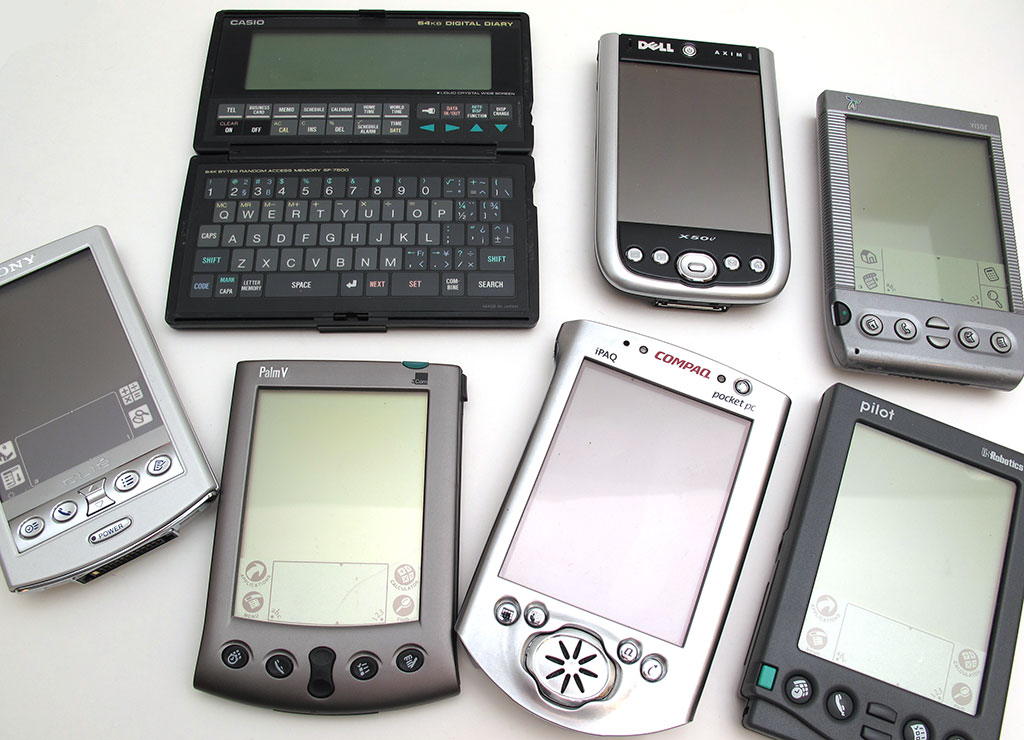
\includegraphics[scale=0.3]{document/chapters/chapter_1/images/pdas.jpg}
    \caption{Examples of PDA devices \cite{is_there_still_a_market_for_pdas}}
    \label{fig:PDAs}
\end{figure}

In 1984 Psion released the first PDA: the Organiser I; the term PDA tho came to existence once in 1992 Apple released the Apple Newton. PDAs started to include telephony capabilities in 1994 with the IBM Simon; this device is particularly important since it can be considered the first smartphone.

Although PDAs had a considerable share of the mobile market (but still dominated by traditional mobile phones), in the mid-2000s PDAs started to be replaced more and more with modern smartphones until they completely replaced them.
Today the term "personal digital assistant" has found a new meaning in the definition of virtual assistants based on speech synthesis (ex: Amazon's Alexa).

Today's mobile devices market not remotely comparable to the market of the PDAs era, reaching exponentially greater number of units sold. Despite this, some experts think that the market is saturated, and it is reaching its peak \cite{smartphones_sales}. One important aspect of today's market is the fact that the number of smartphones currently sold is far greater than the number of PCs sold (that is actually gradually declining) like shown on \textit{figure \ref{fig:global_sales_of_pcs_and_smartphones}}.

\begin{figure}[!ht]
    \centering
    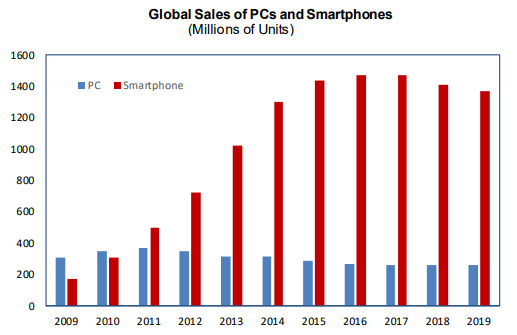
\includegraphics[scale=1]{document/chapters/chapter_1/images/global_sales_of_pcs_and_smartphones.png}
    \caption{Global Sales of PCs and Smartphones from 2009 to 2019 \cite{smartphones_sales}}
    \label{fig:global_sales_of_pcs_and_smartphones}
\end{figure}

\subsection{Technological progress}
TODO also OSs
